\documentclass[border=3]{standalone}

\usepackage{tikz}
\usetikzlibrary{math}

\begin{document}

% ======================================= V
\newcommand{\stickman}[4]{% \stickman ==== V
	\def\x{#1} % center x
	\def\y{#2} % center y
	\def\r{#3} % radius
	\def\name{#4} % name
	\def\xl{\x-\r} % x left
	\def\xr{\x + \r} % x right
	\def\ya{\y-\r} % body upper
	\def\yb{\ya-\r} % arms
	\def\yc{\yb-\r} % legs
	\def\ybd{\yb-0.5*\r} % arms lower
	\def\ycd{\yc-0.5*\r} % legs lower
	
	\draw[
		thick, orange
	]
	(\x, \y) circle (\r) % head
	(\x, \y) node {\name}
	(\x, \ya) -- (\x,\yc) % body
	(\xl, \ybd) -- (\x, \yb) -- (\xr, \ybd) %arms
	(\xl, \ycd) -- (\x, \yc) -- (\xr, \ycd) %arms
	; %
} % \stickman ==== A
% ======================================= A

% ======================================= V
\begin{tikzpicture}

%	% no name
%	\stickman{3}{3}{1} {}
	
	% generation
	\stickman{1}{3}{0.4} {a}
	\stickman{1.8}{4.3}{0.4} {b}
	\stickman{3}{4.8}{0.3} {$c_{i}$}
	\stickman{3.1}{2}{0.4} {}
	\stickman{4}{3}{0.5} {}
	
	% i, j
	\stickman{6}{3}{0.2} {i}
	\stickman{9}{3}{1} {j}
	
	%
%	\stickman{6}{3}{1}{}
%	\stickman{9}{4}{1}{}
%	\stickman{4.5}{4}{1}{}
\end{tikzpicture}
% ======================================= A

\end{document}